The Client Side Application is implemented as a web service to interact with the user and allow the resolution of complex flight requests. The CSA is constructed as a single page application, and is hosted using \textit{heroku}, being publicly available \footnote{The developed CSA has the following URL: \url{https://desolate-castle-31305.herokuapp.com/}}.

The CSA, built using react and redux, evolves around a concept called \textit{state}. The state of the application is stored in the \textit{redux store}, and it contains the relevant information associated to the application at each instance. In the developed application, the state tree is  divided into \textit{requests} and \textit{responses}. Requests are associated to the user input, while responses come from the SSA. The state cycle of the developed application is illustrated in figure \ref{fig:app_state_cycle}.

\begin{figure}[htpb]
  \centering
  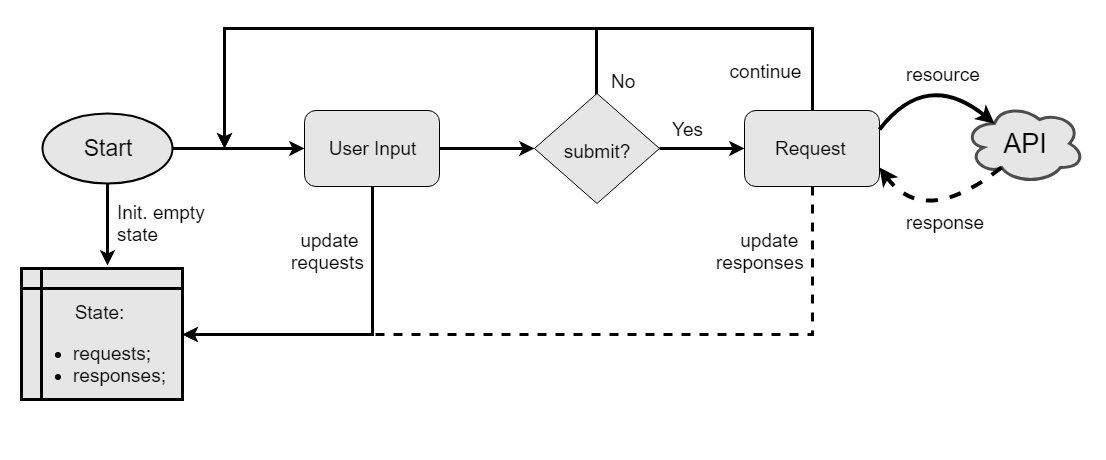
\includegraphics[width=\textwidth]{./Figures/system_implementation/state_flow.png}
  \caption{Block diagram of the state cycle of the Client Side Application.}
  \label{fig:app_state_cycle}  
\end{figure}

To each branch of the state (request and responses) it is associated with a \textit{container} (or a panel view). Containers are top level components, which access the state directly, and call specific components, often using parts of the state as input (props) for them. Thus, the developed application has two main views, as it was proposed in section \ref{sec:csa_design}. There is also a third container, for the map, although it does not have a state branch for itself, but instead derives the necessary information from the other two. 

The complete architecture of the implemented react/redux application, including some of the concepts previously discussed, is illustrated in figure \ref{fig:react_redux_app}. This figure illustrates the top down hierarchy, with a single component in the top of the hierarchy (denoted \textit{app.js}), which instantiates the redux store, and renders the complete application, by invoking the containers which are connected to the relevant presentational components. This figure also illustrates the interaction with the store and with third-party API's. 

\begin{figure}[h!]
  \centering
  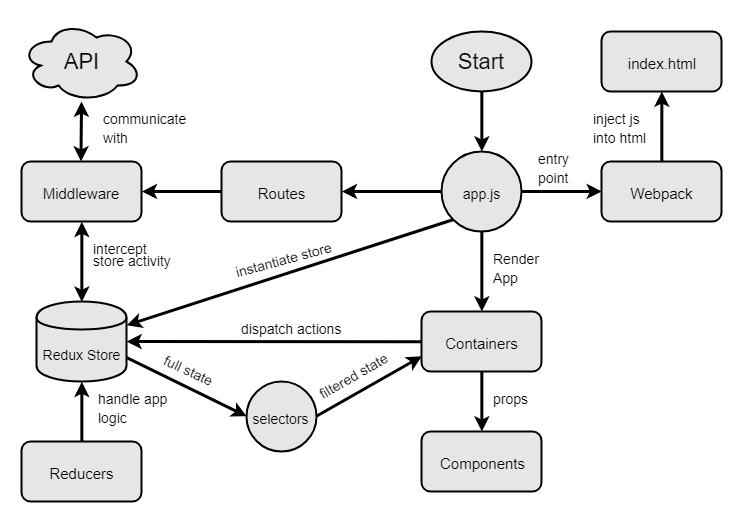
\includegraphics[width=.8\textwidth]{./Figures/system_implementation/react_redux_app.png}
  \caption{Building blocks of an application built using React And Redux.}
  \label{fig:react_redux_app}  
\end{figure}


%Finally, it is important to note that a browser can only render HTML, and the entirety of the application is built using JavaScript. Thus, it is necessary to inject the created JavaScript with all the business and presentation logic, into the HTML file served  to the user. This is usually done by using a package compiler called \textit{Webpack}.

During the remaining of this section, it will be shown how to collect user input (subsection \ref{sec:user_input}) and how to communicate with the SSA  (subsection \ref{sec:api_communication}). Finally, subsection \ref{sec:user_interface_ready} illustrates the developed web application, by presenting some actual screen-shots of it.



